\documentclass{beamer}

\usetheme{CambridgeUS}
\usefonttheme{professionalfonts}

\usepackage{graphicx}
\usepackage[miktex]{gnuplottex}
\ShellEscapetrue
\usepackage{epstopdf}
\usepackage{minted}

\usemintedstyle{manni}
\definecolor{mintedBg}{rgb}{0.98,0.98,0.70}

\begin{document}
\title{A gentle introduction to IR modeling}  
\author{Peter Caspers}
\institute{IKB}
\date{May 23, 2015} 

\frame{\titlepage} 

\frame{\frametitle{Table of contents}\tiny\tableofcontents[hideallsubsections]} 

\section{Introduction}

\frame{\frametitle{What it is all about}
\begin{center}
\Huge Price a derivative contract !
\end{center}
}

\frame{\frametitle{Constraints}
\begin{center}
Do that {\em consistently} with all observable relevant market prices.
\end{center}
}

\frame{\frametitle{Second Thoughts}
What do you mean by ``price'' after all ?
\begin{enumerate}
\item the amount of money that can be realized in the market (``objective'' price)
\item the amount of money that we would require to receive or pay to close the deal (``subjective'' price)
\end{enumerate}
... we will focus on the first kind of price.
}

\frame{\frametitle{Price Adjustments}
\begin{enumerate}
\item CVA
\item DVA
\item FVA
\item KVA
\item MVA
\item TVA
\end{enumerate}
... we exclude all of them in the following.
}

\section{Machinery}

\frame{\frametitle{Randomness}
We need a source of randomness to model the market which is (or appears to be) random.
}

\frame{\frametitle{Stochastic Processes 1}
To model a random observable we assume $X(0)=x_0$ and

\begin{equation}
dX(t,\omega) = \mu(t,\omega) dt + \sigma(t,\omega) dW
\end{equation}

which means, knowing $X(t_0)$ we can evolve forward by

\begin{equation}
X(t_0+\Delta t) \approx X(t_0) + \mu(t) \Delta t + \sigma(t) Z
\end{equation}

with $Z\sim N(0,\Delta t)$ a normal distributed random variable with zero mean and variance $\Delta t$.
}

\frame{\frametitle{Stochastic Processes 2}
The processes above are the processes with {\em continuous} paths.

There is a wider class (Levy processes) which add {\em jumps}. They are also used in finance, but a bit less common.
}

\section{Classification}

\frame{\frametitle{Asset Classes}
Usually we distinguish
\begin{enumerate}
\item Equity
\item FX
\item Interest Rates
\item Credit
\item Inflation
\item Commodity
\end{enumerate}
Today we focus on Interest Rates.
}

\frame{\frametitle{Interest Rate Building Blocks}
Quoted, liquidly traded instruments:
\begin{enumerate}
\item Cash deposits
\item Forward Rate Agreements
\item Vanilla Swaps
\item Short Futures
\item Bond Futures
\end{enumerate}
and in addition options
\begin{enumerate}
\item (Ibor) Caps, Floors
\item Swaptions
\item Futures options
\end{enumerate}
}

\section{Basics}

\frame{\frametitle{Market Models for Options}
Prices for Caps, Floors and Swaptions are quoted using volatilities $\sigma$, assuming a black model for the underlying $F$, either in lognormal style
\begin{equation}
dF = F \sigma dW
\end{equation}
or shifted lognormal style
\begin{equation}
dF = (F+\alpha) \sigma dW
\end{equation}
or in normal style
\begin{equation}
dF = \sigma dW
\end{equation}
all of them having a simple closed form solution (Black formula).
}

\frame{\frametitle{Volatility smile}
Options with different strike and maturity are priced using different volatilities. This seems weird at first sight (at least for the strike direction), but simply means that the Black model is more a quoting convention than a global model.

In strike direction this is referred to as the volatility smile. It simply says that the underlying distirbution is not (shifted) lognormal.
}

\frame{\frametitle{Volatility smile example}

\small SABR 14y/1y implied black lognormal volatilities as of 14-11-2012, input (solid) and Kahale (dashed)

\resizebox{\textwidth}{!}{
\begin{minipage}{1.2\textwidth}
%\centering
% GNUPLOT: LaTeX picture with Postscript
\begingroup
  \makeatletter
  \providecommand\color[2][]{%
    \GenericError{(gnuplot) \space\space\space\@spaces}{%
      Package color not loaded in conjunction with
      terminal option `colourtext'%
    }{See the gnuplot documentation for explanation.%
    }{Either use 'blacktext' in gnuplot or load the package
      color.sty in LaTeX.}%
    \renewcommand\color[2][]{}%
  }%
  \providecommand\includegraphics[2][]{%
    \GenericError{(gnuplot) \space\space\space\@spaces}{%
      Package graphicx or graphics not loaded%
    }{See the gnuplot documentation for explanation.%
    }{The gnuplot epslatex terminal needs graphicx.sty or graphics.sty.}%
    \renewcommand\includegraphics[2][]{}%
  }%
  \providecommand\rotatebox[2]{#2}%
  \@ifundefined{ifGPcolor}{%
    \newif\ifGPcolor
    \GPcolortrue
  }{}%
  \@ifundefined{ifGPblacktext}{%
    \newif\ifGPblacktext
    \GPblacktexttrue
  }{}%
  % define a \g@addto@macro without @ in the name:
  \let\gplgaddtomacro\g@addto@macro
  % define empty templates for all commands taking text:
  \gdef\gplbacktext{}%
  \gdef\gplfronttext{}%
  \makeatother
  \ifGPblacktext
    % no textcolor at all
    \def\colorrgb#1{}%
    \def\colorgray#1{}%
  \else
    % gray or color?
    \ifGPcolor
      \def\colorrgb#1{\color[rgb]{#1}}%
      \def\colorgray#1{\color[gray]{#1}}%
      \expandafter\def\csname LTw\endcsname{\color{white}}%
      \expandafter\def\csname LTb\endcsname{\color{black}}%
      \expandafter\def\csname LTa\endcsname{\color{black}}%
      \expandafter\def\csname LT0\endcsname{\color[rgb]{1,0,0}}%
      \expandafter\def\csname LT1\endcsname{\color[rgb]{0,1,0}}%
      \expandafter\def\csname LT2\endcsname{\color[rgb]{0,0,1}}%
      \expandafter\def\csname LT3\endcsname{\color[rgb]{1,0,1}}%
      \expandafter\def\csname LT4\endcsname{\color[rgb]{0,1,1}}%
      \expandafter\def\csname LT5\endcsname{\color[rgb]{1,1,0}}%
      \expandafter\def\csname LT6\endcsname{\color[rgb]{0,0,0}}%
      \expandafter\def\csname LT7\endcsname{\color[rgb]{1,0.3,0}}%
      \expandafter\def\csname LT8\endcsname{\color[rgb]{0.5,0.5,0.5}}%
    \else
      % gray
      \def\colorrgb#1{\color{black}}%
      \def\colorgray#1{\color[gray]{#1}}%
      \expandafter\def\csname LTw\endcsname{\color{white}}%
      \expandafter\def\csname LTb\endcsname{\color{black}}%
      \expandafter\def\csname LTa\endcsname{\color{black}}%
      \expandafter\def\csname LT0\endcsname{\color{black}}%
      \expandafter\def\csname LT1\endcsname{\color{black}}%
      \expandafter\def\csname LT2\endcsname{\color{black}}%
      \expandafter\def\csname LT3\endcsname{\color{black}}%
      \expandafter\def\csname LT4\endcsname{\color{black}}%
      \expandafter\def\csname LT5\endcsname{\color{black}}%
      \expandafter\def\csname LT6\endcsname{\color{black}}%
      \expandafter\def\csname LT7\endcsname{\color{black}}%
      \expandafter\def\csname LT8\endcsname{\color{black}}%
    \fi
  \fi
  \setlength{\unitlength}{0.0500bp}%
  \begin{picture}(7200.00,5040.00)%
    \gplgaddtomacro\gplbacktext{%
      \csname LTb\endcsname%
      \put(946,704){\makebox(0,0)[r]{\strut{} 0}}%
      \put(946,1156){\makebox(0,0)[r]{\strut{} 0.1}}%
      \put(946,1609){\makebox(0,0)[r]{\strut{} 0.2}}%
      \put(946,2061){\makebox(0,0)[r]{\strut{} 0.3}}%
      \put(946,2513){\makebox(0,0)[r]{\strut{} 0.4}}%
      \put(946,2966){\makebox(0,0)[r]{\strut{} 0.5}}%
      \put(946,3418){\makebox(0,0)[r]{\strut{} 0.6}}%
      \put(946,3870){\makebox(0,0)[r]{\strut{} 0.7}}%
      \put(946,4323){\makebox(0,0)[r]{\strut{} 0.8}}%
      \put(946,4775){\makebox(0,0)[r]{\strut{} 0.9}}%
      \put(1078,484){\makebox(0,0){\strut{} 0}}%
      \put(2509,484){\makebox(0,0){\strut{} 0.05}}%
      \put(3941,484){\makebox(0,0){\strut{} 0.1}}%
      \put(5372,484){\makebox(0,0){\strut{} 0.15}}%
      \put(6803,484){\makebox(0,0){\strut{} 0.2}}%
      \put(176,2739){\rotatebox{-270}{\makebox(0,0){\strut{}black lognormal volatility}}}%
      \put(3940,154){\makebox(0,0){\strut{}strike}}%
    }%
    \gplgaddtomacro\gplfronttext{%
    }%
    \gplbacktext
    \put(0,0){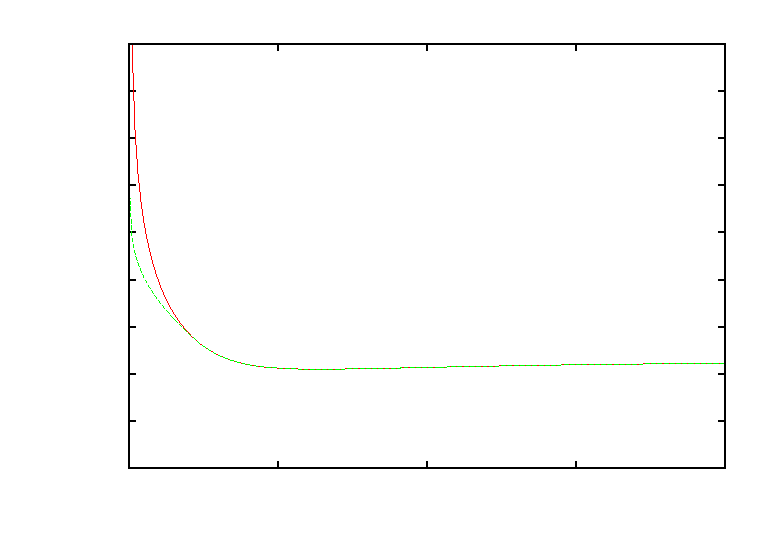
\includegraphics{MF-gnuplottex-fig2}}%
    \gplfronttext
  \end{picture}%
\endgroup

\end{minipage}}

}

\frame{\frametitle{Underlying density}
It is simple to derive the underlying density as
\begin{equation}
\phi(K) = \frac{\partial^2 c}{\partial K^2} \left(K\right)
\end{equation}
for undiscounted call prices. The density is in the natural pricing measure (T-forward measure for caplets, Annuity measure for swaptions). This means you can get (in principle) the market density for an expiry time from a continuum of quoted option prices in strike direction.
}

\frame{\frametitle{No Arbitrage SABR Example}
\resizebox{\textwidth}{!}{
\begin{minipage}{1.5\textwidth}
\begin{figure}
% GNUPLOT: LaTeX picture with Postscript
\begingroup
  \makeatletter
  \providecommand\color[2][]{%
    \GenericError{(gnuplot) \space\space\space\@spaces}{%
      Package color not loaded in conjunction with
      terminal option `colourtext'%
    }{See the gnuplot documentation for explanation.%
    }{Either use 'blacktext' in gnuplot or load the package
      color.sty in LaTeX.}%
    \renewcommand\color[2][]{}%
  }%
  \providecommand\includegraphics[2][]{%
    \GenericError{(gnuplot) \space\space\space\@spaces}{%
      Package graphicx or graphics not loaded%
    }{See the gnuplot documentation for explanation.%
    }{The gnuplot epslatex terminal needs graphicx.sty or graphics.sty.}%
    \renewcommand\includegraphics[2][]{}%
  }%
  \providecommand\rotatebox[2]{#2}%
  \@ifundefined{ifGPcolor}{%
    \newif\ifGPcolor
    \GPcolortrue
  }{}%
  \@ifundefined{ifGPblacktext}{%
    \newif\ifGPblacktext
    \GPblacktexttrue
  }{}%
  % define a \g@addto@macro without @ in the name:
  \let\gplgaddtomacro\g@addto@macro
  % define empty templates for all commands taking text:
  \gdef\gplbacktext{}%
  \gdef\gplfronttext{}%
  \makeatother
  \ifGPblacktext
    % no textcolor at all
    \def\colorrgb#1{}%
    \def\colorgray#1{}%
  \else
    % gray or color?
    \ifGPcolor
      \def\colorrgb#1{\color[rgb]{#1}}%
      \def\colorgray#1{\color[gray]{#1}}%
      \expandafter\def\csname LTw\endcsname{\color{white}}%
      \expandafter\def\csname LTb\endcsname{\color{black}}%
      \expandafter\def\csname LTa\endcsname{\color{black}}%
      \expandafter\def\csname LT0\endcsname{\color[rgb]{1,0,0}}%
      \expandafter\def\csname LT1\endcsname{\color[rgb]{0,1,0}}%
      \expandafter\def\csname LT2\endcsname{\color[rgb]{0,0,1}}%
      \expandafter\def\csname LT3\endcsname{\color[rgb]{1,0,1}}%
      \expandafter\def\csname LT4\endcsname{\color[rgb]{0,1,1}}%
      \expandafter\def\csname LT5\endcsname{\color[rgb]{1,1,0}}%
      \expandafter\def\csname LT6\endcsname{\color[rgb]{0,0,0}}%
      \expandafter\def\csname LT7\endcsname{\color[rgb]{1,0.3,0}}%
      \expandafter\def\csname LT8\endcsname{\color[rgb]{0.5,0.5,0.5}}%
    \else
      % gray
      \def\colorrgb#1{\color{black}}%
      \def\colorgray#1{\color[gray]{#1}}%
      \expandafter\def\csname LTw\endcsname{\color{white}}%
      \expandafter\def\csname LTb\endcsname{\color{black}}%
      \expandafter\def\csname LTa\endcsname{\color{black}}%
      \expandafter\def\csname LT0\endcsname{\color{black}}%
      \expandafter\def\csname LT1\endcsname{\color{black}}%
      \expandafter\def\csname LT2\endcsname{\color{black}}%
      \expandafter\def\csname LT3\endcsname{\color{black}}%
      \expandafter\def\csname LT4\endcsname{\color{black}}%
      \expandafter\def\csname LT5\endcsname{\color{black}}%
      \expandafter\def\csname LT6\endcsname{\color{black}}%
      \expandafter\def\csname LT7\endcsname{\color{black}}%
      \expandafter\def\csname LT8\endcsname{\color{black}}%
    \fi
  \fi
  \setlength{\unitlength}{0.0500bp}%
  \begin{picture}(7200.00,5040.00)%
    \gplgaddtomacro\gplbacktext{%
      \csname LTb\endcsname%
      \put(814,704){\makebox(0,0)[r]{\strut{}-40}}%
      \csname LTb\endcsname%
      \put(814,1213){\makebox(0,0)[r]{\strut{}-30}}%
      \csname LTb\endcsname%
      \put(814,1722){\makebox(0,0)[r]{\strut{}-20}}%
      \csname LTb\endcsname%
      \put(814,2231){\makebox(0,0)[r]{\strut{}-10}}%
      \csname LTb\endcsname%
      \put(814,2740){\makebox(0,0)[r]{\strut{} 0}}%
      \csname LTb\endcsname%
      \put(814,3248){\makebox(0,0)[r]{\strut{} 10}}%
      \csname LTb\endcsname%
      \put(814,3757){\makebox(0,0)[r]{\strut{} 20}}%
      \csname LTb\endcsname%
      \put(814,4266){\makebox(0,0)[r]{\strut{} 30}}%
      \csname LTb\endcsname%
      \put(814,4775){\makebox(0,0)[r]{\strut{} 40}}%
      \csname LTb\endcsname%
      \put(946,484){\makebox(0,0){\strut{} 0}}%
      \csname LTb\endcsname%
      \put(1727,484){\makebox(0,0){\strut{} 0.02}}%
      \csname LTb\endcsname%
      \put(2508,484){\makebox(0,0){\strut{} 0.04}}%
      \csname LTb\endcsname%
      \put(3289,484){\makebox(0,0){\strut{} 0.06}}%
      \csname LTb\endcsname%
      \put(4070,484){\makebox(0,0){\strut{} 0.08}}%
      \csname LTb\endcsname%
      \put(4851,484){\makebox(0,0){\strut{} 0.1}}%
      \csname LTb\endcsname%
      \put(5632,484){\makebox(0,0){\strut{} 0.12}}%
      \csname LTb\endcsname%
      \put(6413,484){\makebox(0,0){\strut{} 0.14}}%
      \put(176,2739){\rotatebox{-270}{\makebox(0,0){\strut{}density}}}%
      \put(3874,154){\makebox(0,0){\strut{}strike}}%
    }%
    \gplgaddtomacro\gplfronttext{%
      \csname LTb\endcsname%
      \put(5816,4602){\makebox(0,0)[r]{\strut{}Hagan (2002)}}%
      \csname LTb\endcsname%
      \put(5816,4382){\makebox(0,0)[r]{\strut{}Doust}}%
    }%
    \gplbacktext
    \put(0,0){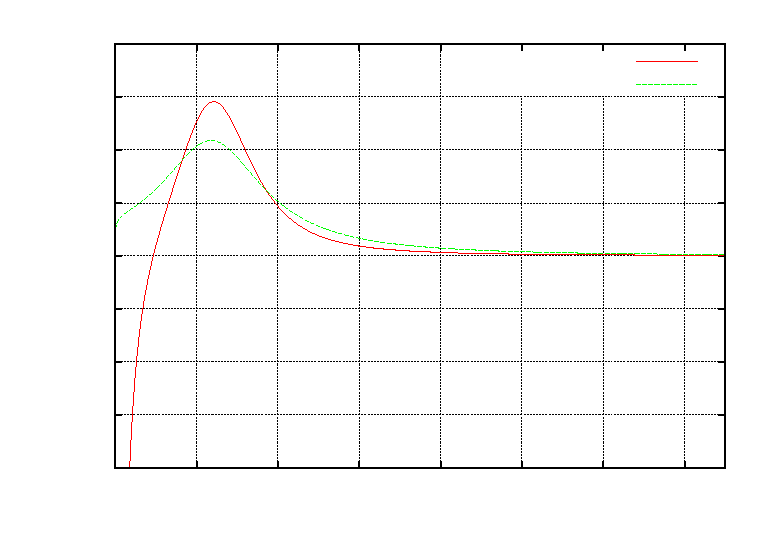
\includegraphics{qlws2014-gnuplottex-fig1}}%
    \gplfronttext
  \end{picture}%
\endgroup

\caption{SABR smile $\alpha=0.02$, $\beta=0.40$, $\nu=0.30$, $\rho=0.30$, $\tau=30.0$, $f=0.03$}
\end{figure}
\end{minipage}}
}

\frame{\frametitle{IR Smile modeling}
In interest rates by far the most common single maturity smile model is the (shifted) SABR model
\begin{eqnarray}
dF(t) &=& (F(t)+\alpha)^\beta \sigma(t) dW \\
d\sigma(t) &=& \sigma(t) \nu dV \\
dV dW &=& \rho dt
\end{eqnarray}
with parameters $\beta$ (skew), $\alpha=\sigma(0)$ (initial level for $\sigma$), $\nu$ (volatility of volatility) and $\rho$ (correlation between forward and vol process).
}

\frame{\frametitle{IR Smile modeling 2}
Other models include
\begin{enumerate}
\item Heston
\item ZABR
\item SVI
\end{enumerate}
}

\frame{\frametitle{Model independent pricing}
Coupons of the following type can be priced only using a no arbitrage argument on today's yield curves:
\begin{enumerate}
\item fixed coupons
\item natural floating rate coupons
\end{enumerate}
Natural means an IBOR - styled coupon with payment date = index accrual period end.
}

\frame{\frametitle{Single maturity model pricing}
Coupons that depend on the distribution of an underlying variable on a single time instance, like
\begin{enumerate}
\item in arrears fixed IBOR coupons
\item capped / floored IBOR coupons
\item CMS coupons
\item CMS Spread Coupons
\end{enumerate}
Usually the effective rate $r$ for coupon estimation is then written
\begin{equation}
r = r_0 + c
\end{equation}
as the sum of the zero volatility forward (i.e. the forward on today's curve) $r_0$ plus a convexity adjustment $c$.
}

\frame{\frametitle{Closed form convexity adjustments}
Assuming a black model for the underlying one can derivate closed form approximations for convexity adjustments
\begin{enumerate}
\item timing adjustments
\item CMS adjustments
\end{enumerate}
}

\frame{\frametitle{Replication CMS convexity adjustments}
To incorporate the market volatility smile into convexity adjustments one uses the underlying density representation and integration by parts together with a simple model.
}

\frame{\frametitle{TSR CMS Coupon Pricers}
A terminal swap rate (TSR) model is given by a mapping $\alpha$
\begin{equation}
\alpha( S(t) ) = \frac{P(t,t_P)}{A(t)}
\end{equation}
where $t_p$ is the coupon payment date and $A(t)$ the annuity of the underlying swap rate $S$. Then (integration by parts) the
npv of a general CMS coupon $A(0) E^A( P(t,t_p) A(t)^{-1} g(S(t)) )$ is given by 
\begin{equation}
A(0)S(0)\alpha(S(0))+\int_{-\infty}^{S(0)} w(k)R(k)dk+\int_{S(0)}^\infty w(k)P(k)dk
\end{equation}
with $t$ begin the fixing date of the coupon, $R$ and $P$ prices of market receiver and payer swaptions and weights $w(s)=\{\alpha(s)g(s)\}''.$
}

\frame{\frametitle{Hagan non parallel shifts model}
In Hagan's classic paper, the model A.4 ``non parallel shifts'' corresponds to the following choice of $\alpha$
\begin{equation}
\alpha( S ) = \frac{S e^{-|h(t_p)-h(t)|x}}{1-\frac{P(0,t_n)}{P(0,t)}e^{-|h(t_n)-h(t)|x}}
\end{equation}
with $t_n$ being the last payment date of the underyling swap and $h(s)-h(t)=\frac{1-e^{-\kappa(s-t)}}{\kappa}$ with a mean reversion parameter $\kappa$ and $x$ implicitly given by
\begin{equation}
S(t) \sum \tau_jP(0,t_j)e^{-|h(t_j)-h(t)|x}+P(0,t_n)e^{-|h(t_n)-h(t)|x} = P(0,t)
\end{equation}
with $\tau_j, t_j$ being the yearfractions and payment dates of the fixed leg of the underlying swap.
}

\frame{\frametitle{Linear TSR model}
The linear terminal swap rate model is defined by

\begin{equation}
\alpha( S ) = a s + b
\end{equation}

$b$ is determined by the no arbitrage condition 

\begin{equation}
P(0,t_p)/A(0) = E^A(P(t,t_p)/A(t)) = a S(0) + b
\end{equation}

$a$ can be specified indirectly via a reversion $\kappa$ by setting

\begin{equation}
a = \frac{\partial}{\partial S(t)}\frac{P(t,t_p)}{A(t)}
\end{equation}

and evaluating the r.h.s. within a one factor gaussian model.
}

\section{HJM class and Hull White Models}

\frame{\frametitle{HJM model class}
With a $d$ - dimensional driving process we have

\begin{equation}
df(t,T) = \sigma_f(t,T)^t \int_t^T \sigma_f(t,u) du dt + \sigma_f(t,T)^t dW(t)
\end{equation}

for instantaneous forward rates $f$ with volatility $\sigma_f$ in the risk neutral measure. The drift is fully specified by the volatilities.

This defines a wide class of interest rate models, on a theoretical level.
}

\frame{\frametitle{Special case: One factor Hull White}
Any gaussian one factor HJM model which satisfies {\it separability}, i.e.
\begin{equation}
\sigma_f(t,T) = g(t)h(T)
\end{equation}

for the instantaneous forward rate volatility with deterministic $g, h>0$, necessarily fulfills

\begin{equation}
dr(t) = (\theta(t) - a(t)r(t)) dt + \sigma(t) dW(t) 
\end{equation}

for the short rate $r$, which means, it is a Hull White one factor model.
}

\frame{\frametitle{The T-forward numeraire}

Set $x(t) := r(t)-f(0,t)$ and fix a horizon $T$, then in the $T$-forward measure the numeraire can be written

\begin{equation}
N(t) = P(t,T) = \frac{P(0,T)}{P(0,t)} e^{-x(t)A(t,T) + B(t,T)}
\end{equation}

with $A, B$ dependent on the model parameters. The Hull White model is called an {\it affine} model.

}

\frame{\frametitle{Smile in the Hull White Model}

\begin{itemize}
\item The distribution of $N(t)$ is lognormal. The shape of the distribution can not
be controlled by any of the model parameters. 
\item For fixed $t$ you can calibrate the model to one market quoted interest rate optoin (typically a caplet or swaption).
\item You can choose the strike of the option, but the rest of the smile is implied by the model.
\end{itemize}

}

\frame{\frametitle{Callable vanilla swaps}

Pricing of callable fix versus Libor swaps may be done in a Hull White model which is calibrated as follows:

\begin{itemize}
\item For each call date find a market quoted swaption which is equivalent to the call right (in some sense, e.g. by matching the npv and its first and second
derivative of the underlying at $E(x(t))$).
\item Calibrate the volatility function $\sigma(t)$ to match the basket of these swaptions.
\item Choose the mean reversion of the model to control serial correlations.
\end{itemize}

}

\frame{\frametitle{Intertemporal correlations}

To understand the role of the reversion parameter assume $\sigma$ and $a$ constant for a moment. Then it is easy to see

\begin{equation}\label{meancorr}
\textnormal{corr}(x(T_1),x(T_2)) = \sqrt{{\frac{e^{2aT_2}-1}{e^{2aT_1}-1}}} = e^{-a(T_2-T_1)} \sqrt{ \frac{1-e^{-2aT_1}}{1-e^{-2aT_2}} }
\end{equation}

which shows that for $a=0$ the correlation is $\sqrt{T_1/T_2}$ and goes to zero if $a\rightarrow\infty$ and to one if $a\rightarrow -\infty$.

}

\frame{\frametitle{Callable cms swaps}

The calll rights in a callable cms swap are options on a swap exchanging cms coupons against fix or Libor rates. Such underlying
swaps are drastically mispriced in the Hull White model in general.

\begin{itemize}
\item cms coupons are replicated using swaptions covering the whole strike continuum $(0,\infty)$
\item The swaption smile in the Hull White model is generally not consistent with the market smile and so are the prices of cms coupons
\end{itemize}

Obviously we need a more flexible model to price such structures

}

\section{Markov Functional Model}

\frame{\frametitle{Model requirements}

The wishlist for the model is as follows

\begin{itemize}
\item We want to be capable of calibrating to a whole smile of (constant maturity) swaptions, not only to one strike, for all fixing dates of the cms coupons. This is to match the coupons of the underlying. 
\item In addition we would like to calibrate to (possibly strike / maturity adjusted) coterminal swaptions to match the options representing the call rights.
\item Finally we need some control over intertemporal correlations, i.e. something operating like the reversion parameter in the Hull White model
\end{itemize}

The idea to do so is to relax the functional dependency between the state variable $x$ and the numeraire $N(t,x)$.
}

\frame{\frametitle{Markov Functional Model}

We start with a markov process driving the dynamics of the model as follows:

\begin{equation}
dx = \sigma(t) e^{at} dW(t)
\end{equation}

and $x(0) = 0$. The intertemporal correlation of the state variable $x$ is the same as for the Hull White model, see (\ref{meancorr}), i.e. the
parameter $a$ can be used to control the correlation just as the reversion parameter in the Hull White model.

}

\frame{\frametitle{The numeraire surface}

The model is operated in the $T$-forward measure, $T$ chosen big enough to cover all cashflows relevant for the actual pricing under consideration. The
link between the state $x(t)$ and the numeraire $P(t,T)$ is given by

\begin{equation}
P(t,T,x) = N(t,x)
\end{equation}

which we allow to be a non parametric surface to have maximum flexibility in calibration.
}

\frame{\frametitle{Calibrating the numeriare surface to market smiles}

The price of a digital swaption paying out an annuity $A(t)$ on expiry $t$ if the swap rate $S(t)\geq K$ in our model is

\begin{equation}\label{modelDigital}
\textnormal{dig}_{\textnormal{model}} = P(0,T) \int_{y^*}^{\infty} \frac{A(t,y)}{P(t,T)} \phi(y) dy
\end{equation} 

where $y^*$ is the strike in the normalized state variable space (the correspondence between $y$ and $S(t)$ is constructed to be monotonic).

}

\frame{\frametitle{Implying the swap rate}

Given the market smile of $S(t)$ we can compute the market price $\textnormal{dig}_\textnormal{mkt}$(K) of digitals for strikes $K$. For given $y^*$
we can solve the equation

\begin{equation}
\textnormal{dig}_\textnormal{mkt}(K) = P(0,T) \int_{y^*}^{\infty} \frac{A(t,y)}{P(t,T)} \phi(y) dy
\end{equation}

for $K$ to find the swap rate corresponding to the state variable value $y^*$. For this $\textnormal{dig}_{mkt}(\cdot)$ should be a monotonic
function whose image is equal to the possible digital prices $(0,A(0)]$. We will revisit this later.

}

\frame{\frametitle{Computing the deflated annuity}

To compute the deflated annuity

\begin{equation}
\frac{A(t)}{P(t,T)} = \sum_{k=1}^n \tau_k \frac{P(t,t_k)}{P(t,T)}
\end{equation}

we observe that

\begin{equation}\label{deflatedZerobond}
\left.\frac{P(t,u)}{P(t,T)}\right|_{y(t)}  = E\left(\frac{1}{P(u,T)} \middle| y(t) \right)
\end{equation}

i.e. we have to integrate the reciprocal of the numeraire at future times. Working backward in time we can assume that
we know the numeraire at these times (starting with $N(T) \equiv 1$).

}

\frame{\frametitle{Converting swap rate to numeraire}

Having computed the swap rate $S(t)$ we have to convert this value to a numeraire value $N(t)$. Since

\begin{equation}
S(t)A(t) + P(t,t^*) = 1
\end{equation}

we get (by division by $N(t)$)

\begin{equation}
N(t) = \frac{1}{S(t)\frac{A(t)}{N(t)} + \frac{P(t,t^*)}{N(t)}}
\end{equation}

all terms on the right hand side computable via deflated zerobonds as shown above. Note that we use a slightly modified swap rate
here, namely one without start delay.

}

\frame{\frametitle{Calibration to a second instrument set}

Up to now we have not made use of the volatility $\sigma(t)$ in the driving markov process of the model. This parameter can be used
to calibrate the model to a second instrument set, however only a single strike can be matched obviously for each expiry. A
typical set up would be
\begin{itemize}
\item calibrate the numeraire to an underlying rate smile, e.g. constant maturity swaptions for cms coupon pricing
\item calibrate $\sigma(t)$ to (standard atm or possibly adjusted) coterminal swaptions for call right calibration
\end{itemize}
Note that after changing $\sigma(t)$ the numeraire surface needs to be updated, too.
}


\frame{\frametitle{Input smile preconditioning}

To ensure a bijective mapping

\begin{equation}
\textnormal{dig}_{\textnormal{mkt}} : (0,\infty) \rightarrow (0,A(0))
\end{equation}

it is sufficient to have an arbitrage free input smile with a $C^1$ call price function. 
It is possible to allow for negative rates and generalize
the interval $(0,\infty)$ to $(-\kappa,\infty)$ with some suitable $\kappa>0$, e.g. $\kappa = 1\%$. In general
input smiles are not arbitrage free, so some preconditioning is advisable, since arbitrageable smiles will break the
numeraire calibration.

}

\begin{frame}[fragile]
\frametitle{A full example: Market Data}
\begin{minted}[fontsize=\tiny]{c++}

#include <ql/quantlib.hpp>
using namespace QuantLib;

int main(int, char * []) {

    try {

        Date refDate(13, November, 2013);
        Date settlDate = TARGET().advance(refDate, 2 * Days);
        Settings::instance().evaluationDate() = refDate;

        Handle<Quote> rateLevel(new SimpleQuote(0.03));
        Handle<YieldTermStructure> yts(
            new FlatForward(refDate, rateLevel, Actual365Fixed()));

        boost::shared_ptr<IborIndex> iborIndex(new Euribor(6 * Months, yts));
        boost::shared_ptr<SwapIndex> swapIndex(
            new EuriborSwapIsdaFixA(10 * Years, yts));

        iborIndex->addFixing(refDate, 0.0200);
        swapIndex->addFixing(refDate, 0.0315);

        Handle<Quote> volatilityLevel(new SimpleQuote(0.30));
        Handle<SwaptionVolatilityStructure> swaptionVol(
            new ConstantSwaptionVolatility(refDate, TARGET(), Following,
                                           volatilityLevel, Actual365Fixed()));

\end{minted}
\end{frame}

\begin{frame}[fragile]
\frametitle{A full example: Cms Swap and Exercise Schedule}
\begin{minted}[fontsize=\tiny]{c++}
        Date termDate = TARGET().advance(settlDate, 10 * Years);

        Schedule sched1(settlDate, termDate, 1 * Years, TARGET(),
                        ModifiedFollowing, ModifiedFollowing,
                        DateGeneration::Forward, false);
        Schedule sched2(settlDate, termDate, 6 * Months, TARGET(),
                        ModifiedFollowing, ModifiedFollowing,
                        DateGeneration::Forward, false);

        Real nominal = 100000.0;
        boost::shared_ptr<FloatFloatSwap> cmsswap(new FloatFloatSwap(
            VanillaSwap::Payer, nominal, nominal, sched1, swapIndex,
            Thirty360(), sched2, iborIndex, Actual360(),
            false,false,1.0,0.0,Null<Real>(),Null<Real>(),1.0,0.00267294));

        std::vector<Date> exerciseDates;
        std::vector<Date> sigmaSteps;
        std::vector<Real> sigma;

        sigma.push_back(0.01);
        for (Size i = 1; i < sched1.size() - 1; i++) {
            exerciseDates.push_back(swapIndex->fixingDate(sched1[i]));
            sigmaSteps.push_back(exerciseDates.back());
            sigma.push_back(0.01);
        }
\end{minted}
\end{frame}

\begin{frame}[fragile]
\frametitle{A full example: Call Right}
\begin{minted}[fontsize=\tiny]{c++}
        boost::shared_ptr<Exercise> exercise(
            new BermudanExercise(exerciseDates));
        boost::shared_ptr<FloatFloatSwaption> callRight(
            new FloatFloatSwaption(cmsswap, exercise));

        std::vector<Date> cmsFixingDates(exerciseDates);
        std::vector<Period> cmsTenors(exerciseDates.size(), 10 * Years);
\end{minted}
\end{frame}

\begin{frame}[fragile]
\frametitle{A full example: Models and Engines}
\begin{minted}[fontsize=\tiny]{c++}
        Handle<Quote> reversionLevel(new SimpleQuote(0.02));

        boost::shared_ptr<NumericHaganPricer> haganPricer(
            new NumericHaganPricer(swaptionVol,
                                   GFunctionFactory::NonParallelShifts,
                                   reversionLevel));
        setCouponPricer(cmsswap->leg(0), haganPricer);

        boost::shared_ptr<MarkovFunctional> mf(new MarkovFunctional(
            yts, reversionLevel->value(), sigmaSteps, sigma, swaptionVol,
            cmsFixingDates, cmsTenors, swapIndex));

        boost::shared_ptr<Gaussian1dFloatFloatSwaptionEngine> floatEngine(
            new Gaussian1dFloatFloatSwaptionEngine(mf));

        callRight->setPricingEngine(floatEngine);
\end{minted}
\end{frame}

\begin{frame}[fragile]
\frametitle{A full example: Calibration Basket}
\begin{minted}[fontsize=\tiny]{c++}
        boost::shared_ptr<SwapIndex> swapBase(
            new EuriborSwapIsdaFixA(30 * Years, yts));

        std::vector<boost::shared_ptr<CalibrationHelper> > basket =
            callRight->calibrationBasket(swapBase, *swaptionVol,
                                         BasketGeneratingEngine::Naive);

        boost::shared_ptr<Gaussian1dSwaptionEngine> stdEngine(
            new Gaussian1dSwaptionEngine(mf));

        for (Size i = 0; i < basket.size(); i++)
            basket[i]->setPricingEngine(stdEngine);
\end{minted}
\end{frame}

\begin{frame}[fragile]
\frametitle{A full example: Model Calibration and Pricing}
\begin{minted}[fontsize=\tiny]{c++}
        LevenbergMarquardt opt;
        EndCriteria ec(2000, 500, 1E-8, 1E-8, 1E-8);
        mf->calibrate(basket, opt, ec);

        std::cout << "model vol & swaption market & swaption model \\\\" << std::endl;
        for (Size i = 0; i < basket.size(); i++) {
            std::cout << mf->volatility()[i] << " & "
                      << basket[i]->marketValue() << " & "
                      << basket[i]->modelValue() << " \\\\" << std::endl;
        }
        std::cout << mf->volatility().back() << std::endl;

        Real analyticSwapNpv = CashFlows::npv(cmsswap->leg(1), **yts, false) -
                               CashFlows::npv(cmsswap->leg(0), **yts, false);
        Real callRightNpv = callRight->NPV();
        Real firstCouponNpv = - cmsswap->leg(0)[0]->amount() * yts->discount(cmsswap->leg(0)[0]->date()) +
                              cmsswap->leg(1)[0]->amount() * yts->discount(cmsswap->leg(1)[0]->date());
        Real underlyingNpv = callRight->result<Real>("underlyingValue") + firstCouponNpv;

        std::cout << "Swap Npv (Hagan)     & " << analyticSwapNpv << "\\\\" << std::endl;
        std::cout << "Call Right Npv (MF)  & " << callRightNpv << "\\\\" << std::endl;
        std::cout << "Underlying Npv (MF)  & " << underlyingNpv << "\\\\" << std::endl;
        std::cout << "Model trace : " << std::endl << mf->modelOutputs() << std::endl;
    }
    catch (std::exception &e) {
        std::cerr << e.what() << std::endl;
        return 1;
    }
}
\end{minted}
\end{frame}

\frame{\frametitle{A full example: Model Calibration (Coterminals)}

\begin{table}[ht]
\begin{tabular}{l | l | l}
model vol & swaption market & swaption model \\ \hline
0.01 & 0.0273707 & 0.0273706 \\
0.0107835 & 0.0337373 & 0.0337373 \\
0.0106409 & 0.0354739 & 0.0354741 \\
0.0109936 & 0.0344716 & 0.0344715 \\
0.0109297 & 0.0315097 & 0.0315096 \\
0.0111361 & 0.0270958 & 0.0270957 \\
0.0111917 & 0.0215014 & 0.0215015 \\
0.0112365 & 0.0150493 & 0.0150493 \\
0.0113241 & 0.00783272 & 0.00783278 \\
0.00998595 & & \\
\end{tabular}
\end{table}

}

\frame{\frametitle{A full example: Pricing}

The expectation is to get a similar price of the underlying cms swap both in
the Markov and the replication model, since both are consistent with the input
swaption smile. Note that the underlying of the swaption is receiving the cms side
while the cms swap is paying.

\begin{table}[ht]
\begin{tabular}{l|l}
Swap Npv (Hagan)     & -0.00\\
Call Right Npv (MF)  & 604.50\\
Underlying Npv (MF)  & 1.00\\
\end{tabular}
\end{table}

The match is very close (0.1 bp times the nominal). It should be noted that from theory
we can not even expect a perfect match since the rate dynamics is not the same
in the Hagan model and the Markov model respectively.
}


\begin{frame}[fragile]
\frametitle{A full example: Benchmarking against Hull White}
We change the code to replace the Markov model with a Hull White model. This is easily done by
\begin{minted}[fontsize=\tiny, bgcolor=mintedBg]{c++}
        std::vector<Date> sigmaSteps2(sigmaSteps.begin(), sigmaSteps.end() - 1);
        std::vector<Real> sigma2(sigma.begin(), sigma.end() - 1);
        boost::shared_ptr<Gsr> gsr(new Gsr(yts,sigmaSteps2,sigma2,reversionLevel->value()));
\end{minted}
and replacing \verb+mf+ by \verb+gsr+ (we could have used a generic name of course...). The calibration now reads
\begin{minted}[fontsize=\tiny, bgcolor=mintedBg]{c++}
        gsr->calibrate(basket, opt, ec, Constraint(), std::vector<Real>(), model->FixedReversions());
\end{minted}
or also
\begin{minted}[fontsize=\tiny, bgcolor=mintedBg]{c++}
        gsr->calibrateVolatilitiesIterative(basket, opt, ec);
\end{minted}

\end{frame}


\begin{frame}[fragile]
\frametitle{A full example: Pricing in the Hull White model}

The fit to the coterminals is exact, just as above (with different model volatilities of course).
The pricing compares ot the Markov model as follows:
\begin{table}[ht]
\begin{tabular}{l|l|l}
Swap Npv (Hagan) & -0.00 & -0.00\\ \hline
 & Markov & Hull White \\ \hline
Call Right Npv   & 604.50 & 1012\\
Underlying Npv   & 1.00 & 657.81\\
\end{tabular}
\end{table}

The underlying and the option are drastically overpriced (both)  by over $60$bp in the Hull White model.
\end{frame}

\begin{frame}[fragile]
\frametitle{A full example: A more realistic smile surface}
Swaption smiles are usually far from being flat. We test the model with a SABR volatility cube
(with constant parameters $\alpha=0.15$, $\beta=0.80$, $\nu=0.20$, $\rho=-0.30$) by setting

\begin{minted}[fontsize=\tiny, bgcolor=mintedBg]{c++}
        Handle<SwaptionVolatilityStructure> swaptionVol(
            new SingleSabrSwaptionVolatility(refDate, TARGET(), Following, 0.15,
                                             0.80, -0.30, 0.20,
                                             Actual365Fixed(), swapIndex));
\end{minted}

\begin{table}[ht]
\begin{tabular}{l|l|l}
Swap Npv (Hagan) & 246.00 & 246.00\\ \hline
 & Markov & Hull White \\ \hline
Call Right Npv   & 696.96 & 1004.79 \\
Underlying Npv   & 259.96 & 648.26 \\
\end{tabular}
\end{table}

Again the underlying and the option is overpriced (by $40$bp resp. $53$bp) in the Hull White model.
In the Markov model the fit is still good ($1.4$bp underlying price difference).
\end{frame}


\begin{frame}[fragile]
\frametitle{A full example: A more realistic smile surface ctd}

Example smile 10y into 10y, $\alpha=0.15$, $\beta=0.80$, $\nu=0.20$, $\rho=-0.30$

\resizebox{\textwidth}{!}{
\begin{minipage}{1.2\textwidth}
% GNUPLOT: LaTeX picture with Postscript
\begingroup
  \makeatletter
  \providecommand\color[2][]{%
    \GenericError{(gnuplot) \space\space\space\@spaces}{%
      Package color not loaded in conjunction with
      terminal option `colourtext'%
    }{See the gnuplot documentation for explanation.%
    }{Either use 'blacktext' in gnuplot or load the package
      color.sty in LaTeX.}%
    \renewcommand\color[2][]{}%
  }%
  \providecommand\includegraphics[2][]{%
    \GenericError{(gnuplot) \space\space\space\@spaces}{%
      Package graphicx or graphics not loaded%
    }{See the gnuplot documentation for explanation.%
    }{The gnuplot epslatex terminal needs graphicx.sty or graphics.sty.}%
    \renewcommand\includegraphics[2][]{}%
  }%
  \providecommand\rotatebox[2]{#2}%
  \@ifundefined{ifGPcolor}{%
    \newif\ifGPcolor
    \GPcolortrue
  }{}%
  \@ifundefined{ifGPblacktext}{%
    \newif\ifGPblacktext
    \GPblacktexttrue
  }{}%
  % define a \g@addto@macro without @ in the name:
  \let\gplgaddtomacro\g@addto@macro
  % define empty templates for all commands taking text:
  \gdef\gplbacktext{}%
  \gdef\gplfronttext{}%
  \makeatother
  \ifGPblacktext
    % no textcolor at all
    \def\colorrgb#1{}%
    \def\colorgray#1{}%
  \else
    % gray or color?
    \ifGPcolor
      \def\colorrgb#1{\color[rgb]{#1}}%
      \def\colorgray#1{\color[gray]{#1}}%
      \expandafter\def\csname LTw\endcsname{\color{white}}%
      \expandafter\def\csname LTb\endcsname{\color{black}}%
      \expandafter\def\csname LTa\endcsname{\color{black}}%
      \expandafter\def\csname LT0\endcsname{\color[rgb]{1,0,0}}%
      \expandafter\def\csname LT1\endcsname{\color[rgb]{0,1,0}}%
      \expandafter\def\csname LT2\endcsname{\color[rgb]{0,0,1}}%
      \expandafter\def\csname LT3\endcsname{\color[rgb]{1,0,1}}%
      \expandafter\def\csname LT4\endcsname{\color[rgb]{0,1,1}}%
      \expandafter\def\csname LT5\endcsname{\color[rgb]{1,1,0}}%
      \expandafter\def\csname LT6\endcsname{\color[rgb]{0,0,0}}%
      \expandafter\def\csname LT7\endcsname{\color[rgb]{1,0.3,0}}%
      \expandafter\def\csname LT8\endcsname{\color[rgb]{0.5,0.5,0.5}}%
    \else
      % gray
      \def\colorrgb#1{\color{black}}%
      \def\colorgray#1{\color[gray]{#1}}%
      \expandafter\def\csname LTw\endcsname{\color{white}}%
      \expandafter\def\csname LTb\endcsname{\color{black}}%
      \expandafter\def\csname LTa\endcsname{\color{black}}%
      \expandafter\def\csname LT0\endcsname{\color{black}}%
      \expandafter\def\csname LT1\endcsname{\color{black}}%
      \expandafter\def\csname LT2\endcsname{\color{black}}%
      \expandafter\def\csname LT3\endcsname{\color{black}}%
      \expandafter\def\csname LT4\endcsname{\color{black}}%
      \expandafter\def\csname LT5\endcsname{\color{black}}%
      \expandafter\def\csname LT6\endcsname{\color{black}}%
      \expandafter\def\csname LT7\endcsname{\color{black}}%
      \expandafter\def\csname LT8\endcsname{\color{black}}%
    \fi
  \fi
  \setlength{\unitlength}{0.0500bp}%
  \begin{picture}(7200.00,5040.00)%
    \gplgaddtomacro\gplbacktext{%
      \csname LTb\endcsname%
      \put(946,704){\makebox(0,0)[r]{\strut{} 0}}%
      \csname LTb\endcsname%
      \put(946,1213){\makebox(0,0)[r]{\strut{} 0.1}}%
      \csname LTb\endcsname%
      \put(946,1722){\makebox(0,0)[r]{\strut{} 0.2}}%
      \csname LTb\endcsname%
      \put(946,2231){\makebox(0,0)[r]{\strut{} 0.3}}%
      \csname LTb\endcsname%
      \put(946,2740){\makebox(0,0)[r]{\strut{} 0.4}}%
      \csname LTb\endcsname%
      \put(946,3248){\makebox(0,0)[r]{\strut{} 0.5}}%
      \csname LTb\endcsname%
      \put(946,3757){\makebox(0,0)[r]{\strut{} 0.6}}%
      \csname LTb\endcsname%
      \put(946,4266){\makebox(0,0)[r]{\strut{} 0.7}}%
      \csname LTb\endcsname%
      \put(946,4775){\makebox(0,0)[r]{\strut{} 0.8}}%
      \csname LTb\endcsname%
      \put(1078,484){\makebox(0,0){\strut{} 0}}%
      \csname LTb\endcsname%
      \put(2223,484){\makebox(0,0){\strut{} 0.02}}%
      \csname LTb\endcsname%
      \put(3368,484){\makebox(0,0){\strut{} 0.04}}%
      \csname LTb\endcsname%
      \put(4513,484){\makebox(0,0){\strut{} 0.06}}%
      \csname LTb\endcsname%
      \put(5658,484){\makebox(0,0){\strut{} 0.08}}%
      \csname LTb\endcsname%
      \put(6803,484){\makebox(0,0){\strut{} 0.1}}%
      \put(176,2739){\rotatebox{-270}{\makebox(0,0){\strut{}implied lognormal black volatility}}}%
      \put(3940,154){\makebox(0,0){\strut{}strike}}%
    }%
    \gplgaddtomacro\gplfronttext{%
    }%
    \gplbacktext
    \put(0,0){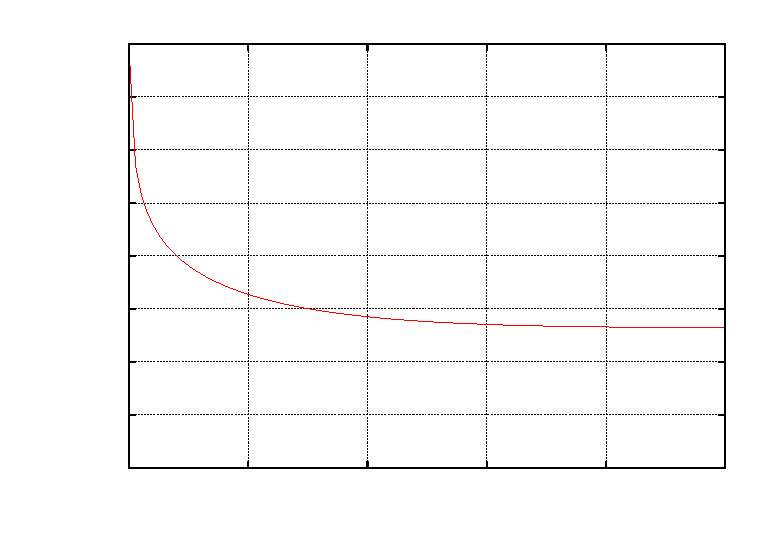
\includegraphics{sabrsmile1}}%
    \gplfronttext
  \end{picture}%
\endgroup

\end{minipage}}
\end{frame}

\begin{frame}[fragile]
\frametitle{A full example: Model diagnostics}
The markov model can generate information on the calibration process with
\begin{minted}[fontsize=\footnotesize, bgcolor=mintedBg]{c++}
std::cout << "Model trace : " << std::endl << mf->modelOutputs() 
          << std::endl;
\end{minted}
The output contains information on
\begin{itemize}
\item numerical model parameters
\item settings for smile preconditioning
\item yield term structure calibration results
\item volatility smile calibration results
\end{itemize}
and can help identifying calibration problems, resp. confirm a successful calibration.
\end{frame}


\begin{frame}[fragile]
\frametitle{A full example: Model diagnostics (model parameters / smile settings)}
\begin{minted}[fontsize=\footnotesize, bgcolor=mintedBg]{c++}
Markov functional model trace output 
Model settings
Grid points y        : 64
Std devs y           : 7
Lower rate bound     : 0
Upper rate bound     : 2
Gauss Hermite points : 32
Digital gap          : 1e-05
Adjustments          : Kahale SmileExp 
Smile moneyness checkpoints: 
\end{minted}
\end{frame}

\begin{frame}[fragile]
\frametitle{A full example: Model diagnostics (yield term structure fit)}
The raw output
\begin{minted}[fontsize=\tiny, bgcolor=mintedBg]{c++}
Yield termstructure fit:
expiry;tenor;atm;annuity;digitalAdj;ytsAdj;marketzerorate;modelzerorate;diff(bp)
November 13th, 2014;10Y;0.03047961644430512;8.267635590910791;1;1;0.03000000000000008;0.03008016185429107;-0.8016185429099432
November 12th, 2015;10Y;0.0304803836917478;8.023747530203391;1;1;0.02999999999999999;0.03003959599137232;-0.395959913723383
[...]
\end{minted}
is meant to be analyzed in another application like office
\resizebox{\textwidth}{!}{
\begin{minipage}{3.0\textwidth}
\begin{figure}
	\centering
		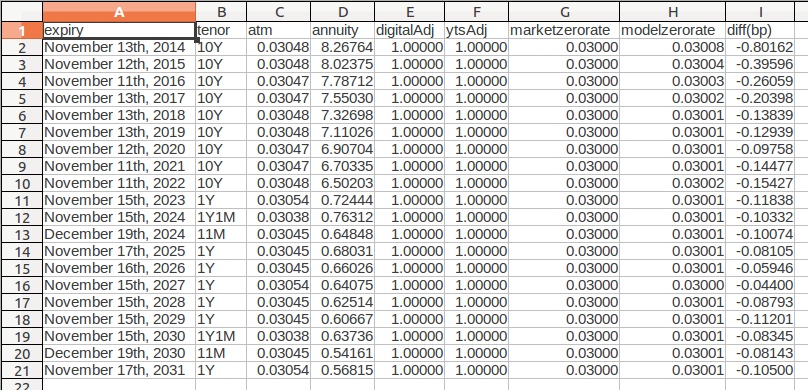
\includegraphics{office_modeltrace1.png}
\end{figure}
\end{minipage}}
\end{frame}

\begin{frame}[fragile]
\frametitle{A full example: Model diagnostics (volatility smile fit)}
\resizebox{\textwidth}{!}{
\begin{minipage}{4.0\textwidth}
\begin{figure}
	\centering
		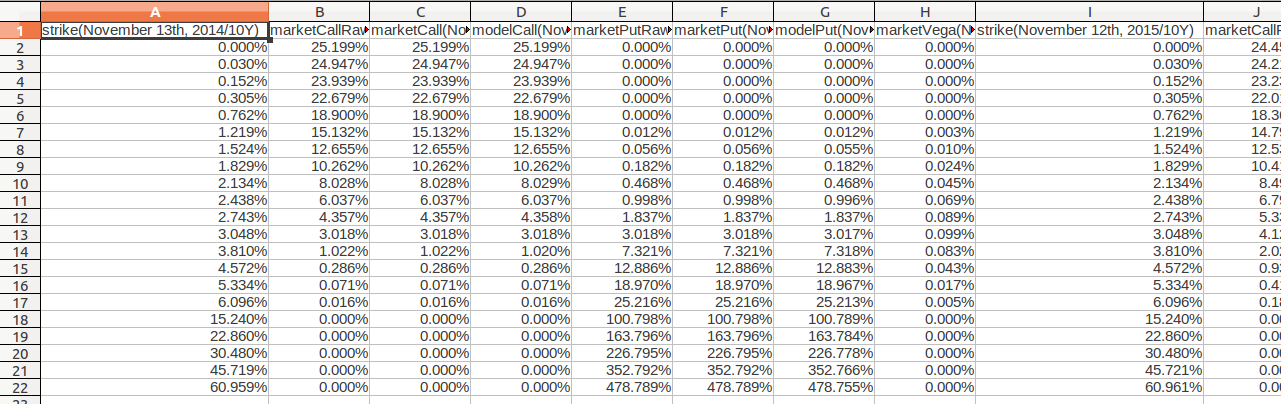
\includegraphics{office_modeltrace2.png}
\end{figure}
\end{minipage}}
\end{frame}


\section{Libor Market Models}

\begin{frame}
\frametitle{Libor Market Models}
Libor Forward Model with displaced diffusion / of Heston type, with forward rate dynamics

\begin{eqnarray}
dF_i(t) &=&  (F_i(t) + d_i) \phi_i \sigma(T_i - t) \sqrt{z(t)} dW_i(t) \\
\sigma(\tau) &=& (a + b\tau) e^{-c\tau} + d
\end{eqnarray} 

with time homogeneous abcd - volatility.
\end{frame}


\begin{frame}
\frametitle{Heston-LFM Correlation Structure}
The correlation structure is given by $dW_i dW_j = \rho_{i,j} dt$ with

\begin{equation}
\rho_{i,j} = \rho_{i,j}^k = \rho_\infty + (1-\rho_\infty) e^{-\beta |(T_i-t_k)-(T_j-t_k)|}
\end{equation}

which allows for a wide range of forward rate correlations through suitable choice of the long term correlation $\rho_\infty$ and the decay factor $\beta$.
\end{frame}


\begin{frame}
\frametitle{Heston-LFM Stochastic Volatility}
The volatility part can be made stochastic by

\begin{equation}
dz(t) = \theta ( 1 - z(t) ) dt + \eta \sqrt{z(t)} dV(t)
\end{equation}

\end{frame}

\begin{frame}
\frametitle{Models}
This is a list of some possible pricing models and their ability to adapt to market parameters.
\begin{table}[ht]
\small
\begin{tabular}{l | l | l | l | l | l}
Model&Murex&QuantLib&Smile&CMS Margin&Decorrelation\\ \hline
HW1F&yes&yes&poor&poor&no \\
MF1F&yes&yes&excellent&excellent&no \\
LFM&under dev&yes&poor&poor&excellent \\
DD-LFM&under dev&yes&good&poor&excellent \\
Heston-LFM&?&yes&good&poor&excellent \\
SABR-LFM&no&no&excellent&excellent&excellent
\end{tabular}
\end{table}

In Particular the 1F models always imply a correlation of 100\% between rates. As we will see, lower
correlation implies a higher option price.
\end{frame}


\section{Summary and Outlook}

\begin{frame}
\frametitle{Summary}
\begin{enumerate}
\item Basic / Single Maturity Models
\item HJM class
\item Hull White Model
\item Markov Functional Model
\item Libor Market Models
\item DD LFM, Heston Volatility
\end{enumerate}
\end{frame}

\begin{frame}
\frametitle{Outlook}
\begin{enumerate}
\item Multi factor gaussian models
\item Quasi gaussian models (allow $g$ above to be stochastic)
\item SABR LFM
\item ...
\end{enumerate}
\end{frame}

\section{Questions}

\begin{frame}[fragile]
\frametitle{Questions / Discussion}
\begin{center}
visit my blog \href{http://quantlib.wordpress.com}{http://quantlib.wordpress.com}
\end{center}
% \resizebox{\textwidth}{!}{
% \begin{minipage}{0.75\textwidth}
% \begin{figure}
% 	\centering
% 		\includegraphics{../../../Pictures/Beaker2.png}
% \end{figure}
% \end{minipage}}
% \\
\end{frame}
\end{document}

